\documentclass[../../../uem_oka_q.tex]{subfiles}

\begin{document}
    図\ref{fig:uem_oka_2025_uni_02_01_q}のように，電極a，bおよび平板cを互いに平行に設置した．%
    bにはスリット$\mathrm{S}_1$が，cにはスリット$\mathrm{S}_2$，$\mathrm{S}_3$がある．%
    $\mathrm{S}_3$の左側には粒子検出器が設置されている．%
    aとbの間の距離は$d$，$\mathrm{S}_2$と$\mathrm{S}_3$の間の距離は$L$とする．

    電極a，bの間に一定の電位差$V$を加え，bと等電位の平板cの右側の領域には%
    磁束密度の大きさが$B$の一様な磁場を印加した．電極bより電極aが高電位である．%
    正の電荷$q$を持ち，質量$m$の粒子を位置Oに静止させ，電極間で加速したところ，%
    $\mathrm{S}_1$，$\mathrm{S}_2$および$\mathrm{S}_3$を通過した後，%
    検出器に到達した．以下の問いに答えよ．ただし，装置は真空中に設置され，%
    重力と地磁気の影響は無視でき，粒子の運動は紙面内に限定されるものとする．

    \begin{enumerate}
        \item%
            電極間で粒子に働く力の大きさを求めよ．$\{d,\,V,\,q,\,m\}$
        \item%
            $\mathrm{S}_1$に到達したときの粒子の速さを求めよ．$\{d,\,V,\,q,\,m\}$
        \item%
            粒子が位置Oから$\mathrm{S}_1$に到達するのに要した時間を求めよ．%
            $\{d,\,V,\,q,\,m\}$
        \item%
            粒子が平板cの右側で描く軌跡を解答欄の図に示せ．
        \item%
            印加されている磁場の向きを答えよ．ただし，座標軸は%
            図\ref{fig:uem_oka_2025_uni_02_01_q}に示すように，$x$軸は平板cに垂直，%
            $z$軸は紙面奥向きを正とする．
        \item%
            印加されている磁場の磁束密度の大きさ$B$を求めよ．\\
            $\{L,\,V,\,q,\,m\}$
    \end{enumerate}

    次に，正の電荷$q$を持ち，質量$\myfraca{m}{2}$の粒子を位置Oに静止させ，%
    電極間で加速した．この粒子は$\mathrm{S}_2$を通過後，$\mathrm{S}_3$を通過することなく%
    平板cに衝突した．%

    \begin{enumerate}[resume]
        \item%
            $\mathrm{S}_2$と衝突点の間の距離は$L$の何倍になるか答えよ．
        \item%
            粒子が$\mathrm{S}_2$を通過してから平板cに衝突するまでに%
            要した時間を求めよ．$\{q,\,m,\,B\}$
    \end{enumerate}
    \newpage
    \noindent
    \begin{minipage}{\linewidth}
        \setlength{\abovecaptionskip}{3pt}
        \centering
            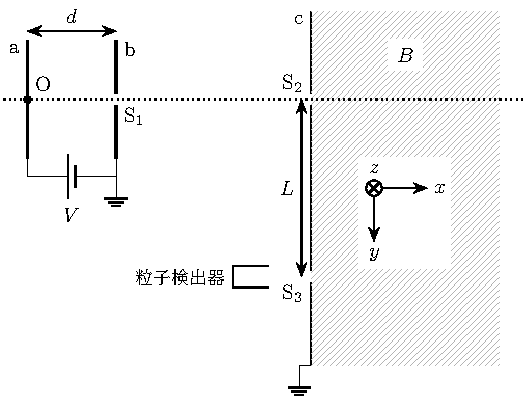
\includegraphics{fig_uem_oka_2025_uni_02/fig_uem_oka_2025_uni_02_01.pdf}
            \captionof{figure}{} \label{fig:uem_oka_2025_uni_02_01_q}
    \end{minipage}
\end{document}